\section{Experiments}
\label{sec:results}

\subsection{Experimental Setup}

\subsubsection{Datasets}

We evaluate on two benchmark PDEs with distinct characteristics:

\textbf{Navier-Stokes equations} describe incompressible fluid dynamics in vorticity form:
\begin{equation}
    \frac{\partial \omega}{\partial t} + u \cdot \nabla \omega = \nu \nabla^2 \omega + f
\end{equation}
where $\omega$ is vorticity, $u$ is velocity, and $\nu$ is viscosity. We use the forced-turbulence benchmark of
Li et al.~\cite{li2020fourier}: a fixed viscosity $\nu = 10^{-3}$ on the unit torus with time-independent
forcing $f(x) = 0.1\left(\sin(2\pi(x_1{+}x_2)) + \cos(2\pi(x_1{+}x_2))\right)$. Each sample maps an input
vorticity field to the vorticity field a fixed time horizon later. The dataset comprises 10\,000 field pairs on
$128 \times 128$ grids, split 8500 training / 500 validation / 1000 test \cite{ns_dataset_zenodo}. Reynolds-number
extrapolation is treated separately in the out-of-distribution study of Experiment~4, which draws on a distinct
parameter-varying dataset. Splitting precedes normalization, and normalization statistics are computed on the
training partition only, so no test information enters training.

\textbf{Darcy Flow} models steady-state flow through porous media:
\begin{equation}
    -\nabla \cdot (k(x) \nabla u) = f
\end{equation}
on the unit square with $u = 0$ on the boundary, where $k(x)$ is a piecewise-constant coefficient field taking
two distinct values and $f = 1$ is a constant source term \cite{li2020fourier}. The dataset comprises 5000
samples on $128 \times 128$ grids, split 4250 training / 250 validation / 500 test \cite{darcy_dataset_zenodo}.

For both PDEs the baseline methods (Deep Ensemble, MC Dropout) were trained under an 80/10/10 split rather
than the 85/5/10 split used for the evidential models, giving them 8000 (Navier-Stokes) and 4000 (Darcy)
training samples. Because both splits are drawn from the same seeded permutation and allocate the same final
10\% of indices to test, \emph{the test partitions are identical} and all numbers in
Table~\ref{tab:baseline_results} are computed on exactly the same held-out samples. The baselines are
nonetheless trained on approximately 6\% fewer samples, a small handicap that should be kept in mind when
reading the accuracy columns.

\subsubsection{Architecture and Training}

All methods use FNO2d with consistent architecture: width = 32, Fourier modes = 12, layers = 4. For evidential variants, the output projection produces 4 channels (NIG parameters) with appropriate activations. MC Dropout applies Dropout2d ($p = 0.1$) after each Fourier layer with $T = 30$ inference passes. Deep Ensemble trains $M = 5$ independent models.

Training uses Adam optimizer with learning rate $\eta = 10^{-3}$, batch size 8, for 20 epochs. Evidential regularization strength $\lambda = 0.01$ for all schemes except KL-Divergence ($\lambda_{\text{KL}} = 0.001$).

\subsubsection{Evaluation Metrics}

We evaluate across three categories:
\begin{itemize}
    \item \textbf{Accuracy}: MSE, MAE, relative $L^2$ error
    \item \textbf{Calibration}: ECE, 95\% coverage, interval width
    \item \textbf{Uncertainty quality}: uncertainty-error correlation, NLL, AUROC (for OOD)
\end{itemize}

\subsection{Experiment 1: Baseline Comparison on Navier-Stokes}

Table~\ref{tab:baseline_results} compares eight UQ methods on Navier-Stokes.

\begin{table*}[htbp]
\centering
\caption{Baseline comparison on Navier-Stokes. Best values in \textbf{bold}.}
\label{tab:baseline_results}
\begin{tabular}{lccccccc}
\toprule
\textbf{Method} & \textbf{MSE} $\downarrow$ & \textbf{MAE} $\downarrow$ & \textbf{rel\_l2} $\downarrow$ & \textbf{ECE} $\downarrow$ & \textbf{Coverage} & \textbf{Correlation} $\uparrow$ & \textbf{NLL} $\uparrow$ \\
\midrule
Linear-Evidence & 0.00162 & 0.0250 & 0.0401 & 0.0046 & 0.932 & 0.518 & -2.196 \\
Log-Barrier & 0.00169 & 0.0260 & 0.0410 & \textbf{0.0038} & 0.924 & 0.611 & -2.152 \\
Inverse-Variance & \textbf{0.00161} & \textbf{0.0251} & \textbf{0.0401} & 0.0045 & 0.934 & \textbf{0.614} & \textbf{-2.200} \\
Exp-Error & 0.00170 & 0.0261 & 0.0412 & 0.0038 & 0.922 & 0.521 & -2.141 \\
L2-Evidence & 0.00163 & 0.0256 & 0.0402 & 0.0066 & \textbf{0.949} & 0.467 & -2.148 \\
KL-Divergence & 0.00149 & 0.0265 & 0.0385 & 0.0303 & 0.993 & 0.437 & -1.787 \\
\midrule
Ensemble \cite{lakshminarayanan2017simple} & 0.00147 & 0.0272 & 0.0382 & 0.0106 & 0.758 & 0.328 & -1.784 \\
MC Dropout \cite{gal2016dropout} & 0.01005 & 0.0758 & 0.1000 & 0.0192 & 0.900 & 0.306 & -0.946 \\
\bottomrule
\end{tabular}
\end{table*}

\textbf{Key findings}: (1) Evidential methods achieve 6$\times$ better MSE than MC Dropout and 2$\times$ better ECE. (2) Inverse-Variance achieves best overall (MSE, correlation, NLL). (3) Log-Barrier/Exp-Error achieve best calibration (ECE = 0.0038). (4) Ensemble shows competitive MSE but severe undercoverage (75.8\%). (5) KL-Divergence produces overwide intervals (0.223) with poor ECE.

\begin{figure*}[htbp]
    \centering
    \begin{subfigure}[b]{0.48\textwidth}
        \includegraphics[width=\textwidth]{img/exp1_ns_uncertainty_aware_sample1.png}
        \caption{Inverse-Variance (best overall: MSE=0.00161, Corr=0.614)}
    \end{subfigure}
    \hfill
    \begin{subfigure}[b]{0.48\textwidth}
        \includegraphics[width=\textwidth]{img/exp1_ns_improved_sample1.png}
        \caption{Log-Barrier (best calibration: ECE=0.0038)}
    \end{subfigure}
    \caption{Navier-Stokes predictions comparing top-performing evidential methods. Left: Inverse-Variance achieves best accuracy and uncertainty correlation. Right: Log-Barrier achieves best calibration with tight confidence intervals.}
    \label{fig:exp1_ns_comparison}
\end{figure*}

\subsection{Experiment 2: Generalization to Darcy Flow}

Table~\ref{tab:darcy_results} evaluates cross-PDE generalization.

\begin{table*}[htbp]
\centering
\caption{Performance comparison on Darcy Flow.}
\label{tab:darcy_results}
\begin{tabular}{lccccccc}
\toprule
\textbf{Method} & \textbf{MSE} $\downarrow$ & \textbf{MAE} $\downarrow$ & \textbf{rel\_l2} $\downarrow$ & \textbf{ECE} $\downarrow$ & \textbf{Coverage} & \textbf{Correlation} $\uparrow$ & \textbf{NLL} $\uparrow$ \\
\midrule
Linear-Evidence & 0.00388 & 0.0313 & 0.0632 & 0.0081 & 0.802 & 0.586 & -1.657 \\
Log-Barrier & \textbf{0.00346} & \textbf{0.0306} & \textbf{0.0597} & 0.0080 & 0.794 & 0.559 & -1.702 \\
Inverse-Variance & 0.00422 & 0.0313 & 0.0659 & \textbf{0.0042} & 0.847 & \textbf{0.659} & \textbf{-1.938} \\
Exp-Error & 0.00389 & 0.0312 & 0.0633 & 0.0069 & 0.813 & 0.544 & -1.652 \\
L2-Evidence & 0.00383 & 0.0316 & 0.0628 & 0.0062 & 0.838 & 0.309 & -1.513 \\
KL-Divergence & 0.00403 & 0.0342 & 0.0644 & 0.0194 & \textbf{0.954} & 0.469 & -1.553 \\
\midrule
Ensemble \cite{lakshminarayanan2017simple} & 0.00652 & 0.0426 & 0.0817 & 0.0061 & 0.652 & 0.461 & -0.827 \\
MC Dropout \cite{gal2016dropout} & 0.01195 & 0.0774 & 0.1107 & 0.0048 & 0.828 & 0.299 & -0.803 \\
\bottomrule
\end{tabular}
\end{table*}

\textbf{Key findings}: (1) Performance rankings transfer across PDEs: Inverse-Variance $\approx$ Log-Barrier $>$ others. (2) Evidential methods dominate---all top-5 MSE are evidential. (3) MC Dropout worst (3.4$\times$ worse MSE, lowest correlation 0.299). (4) Ensemble degrades more severely on Darcy (undercoverage drops to 65.2\%). (5) Coverage systematically lower on Darcy (79--85\%) than Navier-Stokes (92--93\%), indicating PDE-specific calibration may be needed.

\begin{figure*}[htbp]
    \centering
    \begin{subfigure}[b]{0.48\textwidth}
        \includegraphics[width=\textwidth]{img/exp2_darcy_improved_sample1.png}
        \caption{Log-Barrier (best accuracy: MSE=0.00346, rel$L^2$=0.0597)}
    \end{subfigure}
    \hfill
    \begin{subfigure}[b]{0.48\textwidth}
        \includegraphics[width=\textwidth]{img/exp2_darcy_uncertainty_aware_sample1.png}
        \caption{Inverse-Variance (best UQ: ECE=0.0042, Corr=0.659)}
    \end{subfigure}
    \caption{Darcy Flow predictions demonstrating cross-PDE generalization. Performance rankings from Navier-Stokes transfer: Log-Barrier achieves best prediction accuracy while Inverse-Variance maintains superior uncertainty quantification.}
    \label{fig:exp2_darcy_comparison}
\end{figure*}

\subsection{Experiment 3: Physical Consistency of Predicted Uncertainty}

A uncertainty estimate is only actionable for scientific computing if regions of high predicted
uncertainty coincide with regions where the prediction actually violates the governing physics. We
therefore test whether predicted uncertainty is spatially aligned with the PDE residual.

For each test sample we compute the pointwise PDE residual $r_{i,j}$ of the \emph{predicted} field and
correlate it against the pointwise predictive uncertainty $\sqrt{\text{Var}[u_{i,j}]}$ from
Eq.~\eqref{eq:pred_var}. The residual is the strong (pointwise) form of the governing equation---
$|\nabla \cdot (k \nabla \hat{u}) - f|$ for Darcy and the vorticity-transport residual
$|\partial_t \omega + u \cdot \nabla \omega - \nu \nabla^2 \omega|$ for Navier-Stokes, with the time
derivative approximated by a midpoint difference between consecutive snapshots.

Two features of the benchmark datasets in Sec.~\ref{sec:results} make a pointwise strong-form residual
ill-posed, so this experiment is run on matched datasets on which the residual is well-defined. For Darcy,
the benchmark of Table~\ref{tab:darcy_results} uses a piecewise-constant coefficient; there the strong-form
residual is singular at coefficient discontinuities and merely measures proximity to an interface (we
measured a mean residual roughly $17\times$ larger on interface cells). We therefore substitute a
smooth Gaussian-random-field coefficient, on which the reference solutions satisfy the discrete equation to
near machine precision ($\sim\!10^{-5}$). For Navier-Stokes, the benchmark of
Table~\ref{tab:baseline_results} maps an initial field to the solution a long time horizon later, so a
one-step transient residual does not apply; we instead use consecutive vorticity snapshots
$\Delta t = 0.05$ apart from time-resolved trajectories at a single Reynolds number. On ground-truth data
this residual recovers the true time step to within $4\%$, though its irreducible floor is larger than the
Darcy case (about $60\%$ of the characteristic term magnitude, owing to the coarse $\Delta t$ and the
mismatch between the semi-Lagrangian solver and the spectral residual operator); the Navier-Stokes numbers
below should be read with that floor in mind. Both datasets are held distinct from Tables~\ref{tab:baseline_results}
and~\ref{tab:darcy_results}, which this experiment does not claim to reuse.

We report three quantities: the Pearson correlation between residual and
uncertainty across all grid points, the Spearman rank correlation (robust to the heavy-tailed residual
distribution and to the Navier-Stokes floor), and the \emph{residual concentration ratio}---the mean
residual within the top-5\% most uncertain grid points divided by the mean residual over the whole field. A
ratio of 1.0 indicates uncertainty carries no information about physics violation; values substantially
above 1.0 indicate the model flags precisely the regions where it breaks the governing equations.

\begin{table}[htbp]
\centering
\caption{Physical consistency of predicted uncertainty. The concentration ratio is the mean PDE residual
within the top-5\% most uncertain grid points, relative to the field mean; values $>$ 1 indicate
high-uncertainty regions coincide with physics violation. All values are averaged over the test set.}
\label{tab:physics_consistency}
\resizebox{\columnwidth}{!}{%
\begin{tabular}{lcccc}
\toprule
\textbf{Method} & \textbf{PDE} & \textbf{Pearson $r$} $\uparrow$ & \textbf{Spearman $\rho$} $\uparrow$ & \textbf{Conc. Ratio} $\uparrow$ \\
\midrule
Linear-Evidence  & NS & 0.063 & 0.599 & 1.52 \\
Log-Barrier      & NS & 0.067 & 0.564 & 1.50 \\
Inverse-Variance & NS & 0.069 & \textbf{0.633} & 1.58 \\
Exp-Error        & NS & 0.103 & 0.612 & 1.56 \\
L2-Evidence      & NS & \textbf{0.199} & 0.433 & \textbf{1.64} \\
KL-Divergence    & NS & 0.077 & -0.039 & 1.37 \\
\midrule
Linear-Evidence  & Darcy & 0.016 & 0.035 & 1.26 \\
Log-Barrier      & Darcy & 0.005 & 0.027 & 1.19 \\
Inverse-Variance & Darcy & 0.001 & 0.023 & 1.12 \\
Exp-Error        & Darcy & 0.011 & 0.035 & 1.17 \\
L2-Evidence      & Darcy & 0.075 & 0.074 & 1.25 \\
KL-Divergence    & Darcy & 0.085 & 0.091 & 1.18 \\
\bottomrule
\end{tabular}%
}
\end{table}

\textbf{Key findings}: (1) On the transient Navier-Stokes problem, predicted uncertainty is meaningfully
aligned with the PDE residual: the Spearman rank correlation reaches $0.43$--$0.63$ for five of the six
schemes and the concentration ratio is $1.5$--$1.6$, i.e.\ the most uncertain grid points violate the
discrete vorticity balance roughly $1.5\times$ more than the field average. (2) The Pearson correlation is
much weaker ($0.06$--$0.20$) than the Spearman value, consistent with the substantial residual floor on
this dataset: the linear magnitude relationship is buried in noise while the monotonic co-location of
uncertainty and residual survives. (3) KL-Divergence is the consistent outlier (Spearman $-0.04$ on NS),
matching its poorly-structured, over-wide uncertainty seen in Table~\ref{tab:baseline_results}. (4) On
Darcy the correlations are near zero (Spearman $<0.1$, concentration $1.1$--$1.3$): the smooth,
steady problem is solved almost exactly and near-homoscedastically, leaving little spatial residual
structure for the near-uniform uncertainty to track. Physical consistency is therefore not automatic---it
emerges where the prediction problem is genuinely hard and spatially heterogeneous (turbulent transport),
and is essentially absent where the model is uniformly accurate.

\subsection{Experiment 4: Out-of-Distribution Detection}

We distinguish two OOD types: parameter-level (Reynolds number extrapolation) and operator-level (cross-PDE transfer).

\begin{table}[htbp]
\centering
\caption{OOD detection comparison: parameter-level vs. operator-level shift.}
\label{tab:ood_results}
\resizebox{\columnwidth}{!}{%
\begin{tabular}{llccc}
\toprule
\textbf{Train} & \textbf{OOD Test} & \textbf{OOD Type} & \textbf{AUROC} & \textbf{Unc. Ratio} \\
\midrule
NS (Re=1--3k) & NS (Re=5k) & Parameter & 0.547 & 1.1$\times$ \\
\midrule
Navier-Stokes & Darcy Flow & Operator & 1.000 & 378$\times$ \\
Darcy Flow & Navier-Stokes & Operator & 1.000 & 36$\times$ \\
\bottomrule
\end{tabular}%
}
\end{table}

\textbf{Key findings}: (1) Parameter extrapolation shows near-random AUROC (0.547)---the model maintains confidence for Re=5000 despite being outside training range. (2) Cross-PDE transfer achieves perfect AUROC (1.000) in both directions. (3) This suggests parameter extrapolation is \emph{not truly OOD} from an operator perspective---the FNO has learned the underlying physics which applies across Reynolds numbers. (4) Cross-PDE represents genuine operator-level OOD where the governing equations differ fundamentally.

\begin{figure*}[htbp]
    \centering
    \begin{subfigure}[b]{0.32\textwidth}
        \includegraphics[width=\textwidth]{img/exp4_reynolds_ood_roc.png}
        \caption{Parameter OOD (AUROC=0.547)}
    \end{subfigure}
    \hfill
    \begin{subfigure}[b]{0.32\textwidth}
        \includegraphics[width=\textwidth]{img/exp5_cross_pde_ns_to_darcy_roc.png}
        \caption{NS$\rightarrow$Darcy (AUROC=1.000)}
    \end{subfigure}
    \hfill
    \begin{subfigure}[b]{0.32\textwidth}
        \includegraphics[width=\textwidth]{img/exp5_cross_pde_darcy_to_ns_roc.png}
        \caption{Darcy$\rightarrow$NS (AUROC=1.000)}
    \end{subfigure}
    \caption{OOD detection ROC curves. (a) Parameter-level shift (Reynolds extrapolation) yields near-random detection, suggesting learned physics generalizes across parameter ranges. (b,c) Operator-level shift (cross-PDE) achieves perfect separation with 36--378$\times$ uncertainty amplification.}
    \label{fig:exp4_5_ood_roc}
\end{figure*}

% \begin{figure*}[htbp]
%     \centering
%     \begin{subfigure}[b]{0.48\textwidth}
%         \includegraphics[width=\textwidth]{img/exp4_reynolds_ood_uncertainty_dist.png}
%         \caption{Reynolds extrapolation: overlapping distributions}
%     \end{subfigure}
%     \hfill
%     \begin{subfigure}[b]{0.48\textwidth}
%         \includegraphics[width=\textwidth]{img/exp5_cross_pde_ns_to_darcy_uncertainty_dist.png}
%         \caption{Cross-PDE: complete separation}
%     \end{subfigure}
%     \caption{Uncertainty distributions for in-distribution vs OOD samples. Parameter-level OOD shows substantial overlap explaining poor AUROC, while operator-level OOD shows dramatic separation enabling perfect detection.}
%     \label{fig:exp4_5_ood_dist}
% \end{figure*}

\subsection{Experiment 5: Shock Capturing}
\label{sec:exp_shock}

To probe uncertainty on solutions with strong discontinuities, we evaluate on the
two-dimensional compressible Euler equations. We generate 3000 randomized four-quadrant Riemann
problems on a $64 \times 64$ periodic grid with a finite-volume solver (Rusanov flux, MUSCL
reconstruction, SSP-RK2), integrated to $T = 0.15$ so that interacting shocks, contacts and
rarefactions have formed; the solver reproduces the analytic Sod shock-tube state to plotting
accuracy. The evidential FNO maps the full initial state $(\rho, u, v, p)$ to the density field
$\rho(\cdot, T)$. We then measure whether the predicted uncertainty is large at the shocks, using
the gradient magnitude $|\nabla \rho|$ of the true solution as the shock indicator, and report the
Pearson and Spearman correlation between uncertainty and $|\nabla \rho|$ together with the
concentration ratio of Sec.~\ref{sec:results} (mean uncertainty in the top-5\% highest-gradient
cells over the field mean).

\begin{table}[htbp]
\centering
\caption{Shock capturing: alignment of predicted uncertainty with $|\nabla \rho|$ on 2D
compressible Euler. Concentration ratio $\gg 1$ means uncertainty localizes on shocks.}
\label{tab:shock}
\resizebox{\columnwidth}{!}{%
\begin{tabular}{lccc}
\toprule
\textbf{Method} & \textbf{Pearson $r$} $\uparrow$ & \textbf{Spearman $\rho$} $\uparrow$ & \textbf{Shock Conc.} $\uparrow$ \\
\midrule
Linear-Evidence  & 0.646 & 0.565 & 3.88 \\
Log-Barrier      & \textbf{0.660} & \textbf{0.578} & 3.91 \\
Inverse-Variance & 0.654 & 0.571 & 3.90 \\
Exp-Error        & 0.654 & 0.564 & 3.87 \\
L2-Evidence      & 0.623 & 0.572 & 3.88 \\
KL-Divergence    & 0.400 & 0.539 & \textbf{3.95} \\
\midrule
\multicolumn{4}{l}{\textit{Cross-family baselines (sample-disagreement uncertainty)}} \\
MC Dropout       & 0.557 & 0.308 & 3.66 \\
Deep Ensemble    & 0.561 & 0.372 & 3.57 \\
\bottomrule
\end{tabular}%
}
\end{table}

\textbf{Key findings}: (1) On shocks the alignment is strong and uniform: every scheme concentrates
uncertainty by a factor of $3.9\times$ on the sharpest-gradient cells, and the Pearson correlation
with $|\nabla \rho|$ is $0.62$--$0.66$ for five of six schemes. (2) The model flags discontinuities
as uncertain because they are exactly where the initial-to-final map is hardest to learn---sharp
features coincide with large prediction error, so difficulty and error agree. (3) KL-Divergence has
the weakest linear correlation ($0.40$) but the same concentration, consistent with its
over-dispersed uncertainty elsewhere in this study. (4) The behavior is not specific to the
evidential parameterization: the two sampling-based families concentrate uncertainty on shocks as
well ($3.6$--$3.7\times$, Pearson $0.56$), confirming that ``hard local structure reads as
uncertain'' is a property shared across uncertainty methods rather than an artifact of the NIG head.

\subsection{Experiment 6: Long-Horizon Rollout}
\label{sec:exp_rollout}

Scientific surrogates are often applied autoregressively, so we test whether predicted uncertainty
grows as rollout error accumulates. Using the PDEArena Navier-Stokes benchmark \cite{gupta2022pdearena}
(128$\times$128 velocity trajectories), we convert to vorticity and train the evidential FNO on the
one-step map $\omega^{t} \mapsto \omega^{t+1}$. At test time we roll the model out autoregressively
from $\omega^0$ over the full trajectory and record, at each step, the relative $L^2$ error against
the ground truth and the mean predicted uncertainty. A well-calibrated surrogate should become
\emph{more} uncertain as it drifts. We report the error at the final step, the error and uncertainty
growth ratios (last step over first), and the Pearson correlation between the per-step error and
uncertainty curves.

\begin{table}[htbp]
\centering
\caption{Long-horizon rollout on Navier-Stokes. \texttt{unc.\ growth} $<1$ means uncertainty
\emph{shrinks} during rollout; a negative \texttt{step corr} means uncertainty moves opposite to error.}
\label{tab:rollout}
\resizebox{\columnwidth}{!}{%
\begin{tabular}{lcccc}
\toprule
\textbf{Method} & \textbf{Final err.} & \textbf{Err.\ growth} & \textbf{Unc.\ growth} & \textbf{Step corr.} \\
\midrule
Linear-Evidence  & 1.09 & 1.42 & 0.14 & $-0.995$ \\
Log-Barrier      & 1.11 & 1.46 & 0.16 & $-0.984$ \\
Inverse-Variance & 1.14 & 1.50 & 0.16 & $-0.976$ \\
Exp-Error        & 1.22 & 1.55 & 0.08 & $-0.806$ \\
L2-Evidence      & 1.15 & 1.51 & 0.11 & $-0.937$ \\
KL-Divergence    & 1.17 & 1.57 & 0.17 & $-0.930$ \\
\midrule
\multicolumn{5}{l}{\textit{Cross-family baselines (sample-disagreement uncertainty)}} \\
MC Dropout       & 1.00 & 1.41 & 0.17 & $-0.918$ \\
Deep Ensemble    & 0.98 & 1.43 & 0.09 & $-0.905$ \\
\bottomrule
\end{tabular}%
}
\end{table}

\begin{figure}[htbp]
    \centering
    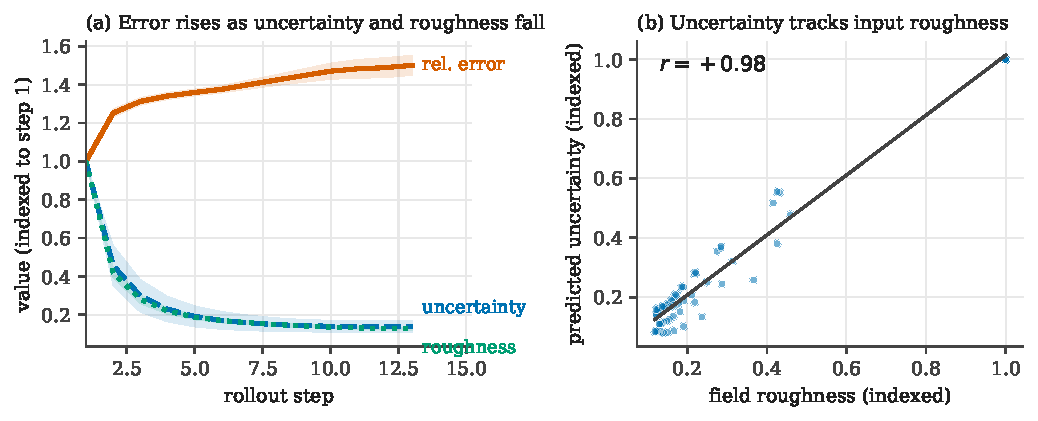
\includegraphics[width=\columnwidth]{img/rollout_drift.pdf}
    \caption{Mechanism of the rollout failure, averaged over the six schemes.
    (a) Indexed to the first rollout step, the relative error rises while the predicted
    uncertainty and the field roughness ($\overline{|\nabla \omega|}$) collapse together to
    $\sim\!13\%$. (b) Pooled over all schemes and steps, predicted uncertainty is an almost
    deterministic increasing function of the input field's roughness ($r = 0.98$). The model's
    uncertainty tracks how rough the current input looks, not how wrong the prediction is.}
    \label{fig:rollout}
\end{figure}

\textbf{Key findings}: (1) The result is the mirror image of Experiment 5 and is uniform across
schemes: as rollout error grows by $\sim\!1.5\times$, predicted uncertainty \emph{collapses} to
$8$--$17\%$ of its initial value, anti-correlated with error at a mean step correlation of $-0.94$.
(2) The model becomes more confident precisely as it drifts further from the true dynamics---the
same over-confidence-under-shift failure observed for parameter extrapolation in
Experiment~4. (3) The mechanism unifies Experiments 5 and 6: the predicted uncertainty is a
pointwise, learned function of the \emph{current input's local structure}, calibrated only
in-distribution. Sharp inputs (shocks) are read as uncertain and are indeed hard, so uncertainty
tracks error; but the FNO's spectral smoothing drives the autoregressive state toward blurred,
low-gradient fields that the model reads as easy---smooth yet increasingly wrong---so uncertainty
falls exactly when it should rise. Fig.~\ref{fig:rollout} makes this quantitative: across all six
schemes the predicted uncertainty tracks the field roughness $\overline{|\nabla \omega|}$ at a mean
correlation of $0.99$ (while roughness itself falls to $\sim\!13\%$ and anti-correlates with error),
so the reported uncertainty is effectively a readout of input smoothness rather than of prediction
error. (4) As in Experiment~5, the failure is cross-family, not evidential-specific: MC Dropout and
Deep Ensemble both collapse under rollout (uncertainty growth $0.17\times$ and $0.09\times$; step
correlation $-0.918$ and $-0.905$) and their uncertainty tracks input roughness just as tightly
(corr $0.985$ and $0.984$). The sampling-based methods estimate uncertainty from prediction
\emph{disagreement}, yet they too grow confident as the rollout state smooths, because every member
reads the same blurred input as easy. Faithful uncertainty under distribution shift therefore requires
a mechanism sensitive to global departure from the training manifold, not the pointwise evidence
used here (Sec.~\ref{sec:limitations})---and this requirement is shared by the sampling-based
baselines, not unique to evidential learning.

\subsection{Experiment 7: Architectural Ablation}

We ablate key components from the Log-Barrier evidential FNO using 3500 sample as train set and 1500 sample for test set. The Baseline row refers to the full Log-Barrier model with all default components intact, serving as the reference for comparison.

\begin{table}[htbp]
\centering
\caption{Ablation study. NaN indicates model failure (constant predictions).}
\label{tab:ablation}
\resizebox{\columnwidth}{!}{%
\begin{tabular}{lcccc}
\toprule
\textbf{Variant} & \textbf{MSE} $\downarrow$ & \textbf{rel\_l2} $\downarrow$ & \textbf{Calib.} $\downarrow$ & \textbf{Corr.} $\uparrow$ \\
\midrule
Baseline & \textbf{0.00194} & 0.0442 & 0.029 & 0.455 \\
\midrule
no\_skip\_connections & 0.996 & 1.000 & 0.339 & NaN \\
fourier\_only & 0.996 & 1.000 & 0.374 & NaN \\
no\_activations & 0.040 & 0.201 & 0.105 & 0.416 \\
with\_batch\_norm & 0.004 & 0.066 & 0.038 & 0.420 \\
\midrule
shallow\_heads & 0.002 & 0.045 & 0.029 & 0.447 \\
linear\_heads & 0.003 & 0.057 & 0.037 & 0.457 \\
with\_residual & 0.002 & \textbf{0.043} & \textbf{0.028} & 0.452 \\
\bottomrule
\end{tabular}%
}
\end{table}

\textbf{Key findings}: (1) Skip connections are critical---removing causes catastrophic failure (MSE $\approx$ 1.0). (2) Pure Fourier convolution without local components also fails completely. (3) Activations are necessary---removal causes 20$\times$ MSE degradation. (4) Batch normalization harms performance (2.2$\times$ worse). (5) Evidential head complexity matters little---shallow or linear heads maintain similar performance with fewer parameters. (6) Global residual connections provide modest improvement ($\sim$5\%).

\textbf{Design recommendations}: Required---skip connections, GELU activations. Recommended---global residuals. Optional---shallow evidential heads. Avoid---batch normalization.

\begin{figure*}[htbp]
    \centering
    \begin{subfigure}[b]{0.48\textwidth}
        \includegraphics[width=\textwidth]{img/exp6_ablation_performance.png}
        \caption{Prediction accuracy (MSE, rel$L^2$)}
    \end{subfigure}
    \hfill
    \begin{subfigure}[b]{0.48\textwidth}
        \includegraphics[width=\textwidth]{img/exp6_ablation_calibration.png}
        \caption{Calibration metrics}
    \end{subfigure}
    \caption{Architectural ablation results. Removing skip connections or using pure Fourier convolution causes catastrophic failure (MSE$\approx$1.0). Batch normalization degrades performance 2.2$\times$. Evidential head complexity (shallow vs. linear) has minimal impact on final performance.}
    \label{fig:exp6_ablation}
\end{figure*}